\section{Introducción}
En este documento vamos a tratar el ``esquema de criptografía visual'' propuesto
por \textsl{Moni Naor} y \textsl{Adi Shamir}\cite{naor_shamir}\ y una extensión
del mismo donde cambiamos píxeles por letras\cite{articulo_base}. También
veremos algunos detalles de las implementaciones de ambos.

Esta técnica permite encriptar una imagen, y desencriptarla mecánicamente, sin
la intervención de un ordenador \cite{wikipedia}. Fue propuesta por \textsl{Moni
Naor} y \textsl{Adi Shamir} en 1994 como una representación visual del ``esquema
de secreto compartido'' propuesto por Shamir en 1979
\cite{articulo_base}\cite{articulo_esp}.

Como se aprecia en el esquema de la figura \ref{fig:esquema}, una imágen se
cifra en $N$ sombras. Harán falta un mínimo de $K$ sombras para que, al
superponerlas, se revele el secreto. Un número de sombras menor que $K$ no
revela ninguna información sobre la imagen original (\reffig{fig:ejemplo33}).

\begin{figure}[ht]
	\centering
	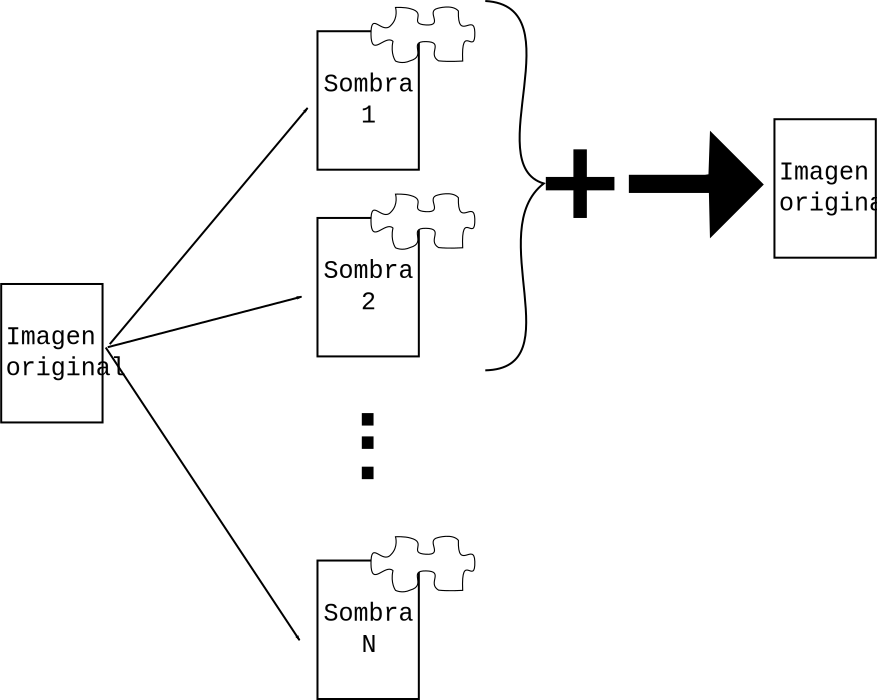
\includegraphics[width=0.8\textwidth]{images/esquema}
	\caption{Esquema de cifrado y descrifrado}
	\label{fig:esquema}
\end{figure}

\begin{figure}[Hp]
	\centering
	\begin{subfigure}[t]{0.3\textwidth}
		\centering
		\includegraphics[width=\textwidth]{images/shade00}
		\caption{Sombra 1}
	\end{subfigure}
	\hspace{0.5cm}
	\begin{subfigure}[t]{0.3\textwidth}
		\centering
		\includegraphics[width=\textwidth]{images/shade0y1}
		\caption{Sombra 1 y 2}
	\end{subfigure}
	\\
	\begin{subfigure}[t]{0.3\textwidth}
		\centering
		\includegraphics[width=\textwidth]{images/shade01}
		\caption{Sombra 2}
	\end{subfigure}
	\hspace{0.5cm}
	\begin{subfigure}[t]{0.3\textwidth}
		\centering
		\includegraphics[width=\textwidth]{images/shade0y2}
		\caption{Sombras 1 y 3}
	\end{subfigure}
	\\
	\begin{subfigure}[t]{0.3\textwidth}
		\centering
		\includegraphics[width=\textwidth]{images/shade02}
		\caption{Sombra 3}
	\end{subfigure}
	\hspace{0.5cm}
	\begin{subfigure}[t]{0.3\textwidth}
		\centering
		\includegraphics[width=\textwidth]{images/shade1y2}
		\caption{Sombras 2 y 3}
	\end{subfigure}
	\\
	\begin{subfigure}[t]{0.3\textwidth}
		\centering
		\includegraphics[width=\textwidth]{images/original}
		\caption{Resultado (sombras 1, 2 y 3)}
	\end{subfigure}
	\hspace{0.5cm}
	\begin{subfigure}[t]{0.3\textwidth}
		\centering
		\includegraphics[width=\textwidth]{images/result}
		\caption{Imagen original}
	\end{subfigure}
	\caption{Ejemplo de supersposición de sombras en un esquema (3,3)}
	\label{fig:ejemplo33}
\end{figure}
